\documentclass[a4paper]{article}

\usepackage[UTF8]{ctex}
\usepackage[a4paper,margin=1in]{geometry}
\usepackage{graphicx}
\usepackage{float}
\usepackage{listings}
\usepackage{longtable}
\usepackage{booktabs}
\usepackage{hyperref}
\usepackage{fancyhdr}
\usepackage{lastpage}
\usepackage{color}
\usepackage{xcolor}
\usepackage{indentfirst}
\setlength{\parindent}{2em}
\usepackage{zhnumber}
\usepackage[dvipsnames]{xcolor}
\usepackage{amsmath}
\usepackage{multimedia}
\usepackage{qrcode}
\usepackage[most]{tcolorbox}
\usepackage{amssymb}
\usepackage{algorithm}
\usepackage{algorithmic}
%\newcommand{\college}{中山大学计算机学院}
\newcommand{\projname}{计算机图形学|大作业}
\newcommand{\reporttitle}{基于OpenGL的3D象棋系统设计与实现}
\newcommand{\authorname}{熊彦钧、马福泉、吴深荣}
\newcommand{\major}{计算机科学与技术}
\newcommand{\adviser}{陶钧}
\newcommand{\startdate}{2025年12月14日}
\newcommand{\labenddate}{2026年1月17日}
\newcommand{\labroom}{B402}

\setlength{\headheight}{24pt} % Fix fancyhdr warning

\pagestyle{fancy} % 使用 fancyhdr 风格
\fancyhf{}      % 清空默认的页眉页脚

% 设置页眉
\fancyhead[L]{\kaishu \projname}      % 左侧页眉显示项目名称
\fancyhead[C]{\kaishu \reporttitle}    % 中间页眉显示报告标题
\fancyhead[R]{\kaishu \authorname} % 右侧页眉显示作者姓名

% 设置页脚
\fancyfoot[C]{第 \thepage 页，共 \pageref{LastPage} 页} % 中间页脚显示页码

% 去除页眉页脚与正文之间的分隔线
\renewcommand{\headrulewidth}{0.4pt}
\renewcommand{\footrulewidth}{0pt}

% 设置文档背景颜色
\definecolor{mybgcolor}{RGB}{0, 0, 0} % 定义背景颜色
\definecolor{NavyBlue}{RGB}{0,0,128} % 添加颜色定义
% \pagecolor{mybgcolor} % 设置背景颜色

\lstset{
    basicstyle=\ttfamily\small,
    commentstyle=\color{gray}\itshape,
    keywordstyle=\color{NavyBlue}\bfseries,
    stringstyle=\color{Red},
    breaklines=true,
    frame=shadowbox,
    rulesepcolor=\color{gray!20},
    numbers=left,
    numberstyle=\tiny\color{gray},
    tabsize=4,
    showstringspaces=false,
    captionpos=b,
    language=C++,
    morekeywords={glm, vec3, vec2, mat4, GLuint, uniform, layout, in, out}
}

\usepackage{tikz}
\usetikzlibrary{shapes.geometric, arrows, positioning, shadows, calc, fit}

\begin{document}

% 封面
\begin{titlepage}
    \centering
    

    
\includegraphics[width=10cm]{img/SYSULogo.png}

    \vspace{1em}
    %{\Large \college \par}
    \vspace{1em}
    {\Large \kaishu \projname \par}
    \vspace{3em}

    

    
    {\fontsize{40pt}{42pt}\kaishu \selectfont \boldmath \reporttitle\par}
    \vspace*{\fill}

    \begin{center}
    {\Large
    \makebox[5em][s]{姓名}:\underline{\makebox[15em][c]{\kaishu \authorname}}\\[1em]
    \makebox[5em][s]{专业}:\underline{\makebox[15em][c]{\kaishu \major}}\\[1em]
    \makebox[5em][s]{课程教师}:\underline{\makebox[15em][c]{\kaishu \adviser}}\\[1em]
    \makebox[5em][s]{起始日期}:\underline{\makebox[15em][c]{\kaishu \startdate}}\\[1em]
    \makebox[5em][s]{结束日期}:\underline{\makebox[15em][c]{\kaishu \labenddate}}\\[1em]
    \makebox[5em][s]{实验地点}:\underline{\makebox[15em][c]{\kaishu \labroom}}
    }
    \end{center}

    \vspace*{\fill}
\end{titlepage}

% 目录
\tableofcontents

\newpage

% 实验报告正文开始

\begin{abstract}
本项目基于 OpenGL 3.3 Core Profile 架构，设计并实现了一个高真实感的 3D 中国象棋对弈系统。项目摒弃了传统的固定管线开发模式，完全采用现代可编程管线技术（Programmable Pipeline），在保证实时渲染性能（稳定 60 FPS+）的前提下，集成了多项高级图形学特性。

在视觉表现上，系统实现了基于 Phong 模型的复杂光照计算、两遍法（Two-Pass）阴影映射（Shadow Mapping）以及基于等距柱状投影（Equirectangular Projection）的高动态范围天空盒。在工程实践方面，针对 Windows 环境下 C++ 开发中常见的中文路径资源加载痛点，本项目引入了 Windows Imaging Component (WIC) 替代传统的 \texttt{stb\_image} 库，利用 COM 组件技术彻底解决了多语言环境下的路径编码问题。此外，项目探索了程序化建模（Procedural Modeling）技术，通过三角函数参数方程动态生成具有自然扰动效果的石桌与石凳模型，相比静态网格加载降低了显存占用与磁盘 I/O 开销。

交互方面，系统实现了基于逆矩阵变换的射线投射（Ray Casting）算法，支持精确的 3D 空间拾取与棋子移动。实验结果表明，该系统在视觉保真度、交互流畅性及代码健壮性方面均达到了预期目标，是对计算机图形学理论与工程实践的一次深度整合。

\textbf{关键词：} OpenGL, Shadow Mapping, WIC, Ray Casting, Procedural Modeling, Skybox, GLSL
\end{abstract}
\newpage

\section{项目介绍}

\subsection{项目背景与技术调研}
随着计算机图形硬件的飞速发展，图形渲染技术经历了从早期的固定管线（Fixed Function Pipeline）到现代可编程管线（Programmable Pipeline）的范式转移。早期的 OpenGL 版本依赖预定义的渲染状态，虽然易于入门，但难以实现复杂且独特的光影效果。现代 OpenGL（3.3+）通过引入 GLSL 着色器语言，赋予了开发者直接控制 GPU 顶点与片元处理阶段的能力，使得基于物理的渲染（PBR）、动态阴影和复杂材质表现成为可能。

在 3D 棋类仿真应用的开发中，核心挑战在于如何在一个有限的交互空间内，提供视觉真实感与流畅的操作体验。这不仅要求系统具备高精度的几何建模和实时光影计算能力（如阴影遮挡、环境反射），还要求解决工程实践中的资源管理难题（如多语言环境下的文件加载）以及三维空间中的精确交互（如鼠标拾取）。本项目正是在此背景下，基于 OpenGL 3.3 Core Profile 架构进行的一次技术实践。

\subsection{项目概述}
本项目旨在设计并实现一个高真实感、强交互性的 3D 中国象棋对弈系统。系统涵盖了从底层引擎搭建到上层逻辑实现的完整开发流程，主要技术特性如下：

\begin{enumerate}
    \item \textbf{沉浸式渲染环境}：
    系统摒弃了简单的纯色背景，实现了基于等距柱状投影（Equirectangular Projection）的高动态范围天空盒（Skybox），配合 \texttt{z=w} 深度优化技术，构建了无缝的自然环境背景。同时，引入了改进的 Phong 光照模型，实现了环境光、漫反射与高光反射的实时计算。
    \item \textbf{高级阴影渲染}：
    为了增强场景的体积感，项目实现了两遍法（Two-Pass）阴影映射技术。通过从光源视角生成深度贴图（Depth Map），并在主渲染通道中进行深度比对，生成了动态阴影。此外，应用了 PCF（Percentage-Closer Filtering）采样算法，有效解决了阴影边缘锯齿和自遮挡（Shadow Acne）问题，实现了软阴影效果。
    \item \textbf{工程化资源管理}：
    针对 Windows 平台 C++ 开发中常见的中文路径资源加载痛点，项目创新性地封装了 Windows Imaging Component (WIC) 接口，替代了传统的 \texttt{stb\_image} 库。利用 COM 组件技术，彻底解决了包含中文字符纹理（如“红车.png”）的加载与解码问题。
    \item \textbf{程序化与参数化建模}：
    项目探索了程序化建模（Procedural Modeling）技术，不依赖外部模型文件，而是通过数学参数方程动态生成几何体。特别是对于石桌与石凳，引入了正弦波扰动算法，模拟了自然石材表面的不规则起伏，兼顾了视觉细节与存储效率。
    \item \textbf{精确交互逻辑}：
    实现了基于逆矩阵变换的射线投射（Ray Casting）算法，能够将 2D 屏幕空间的鼠标点击精确映射到 3D 世界坐标系，实现了棋子的精准拾取、悬浮反馈与落子操作。
\end{enumerate}

\subsection{项目分工}

为了保证项目的高效推进，小组成员根据各自的技术专长进行了明确的分工与协作。

\begin{tcolorbox}[colback=yellow!10!white, colframe=brown!70!black, title=\textbf{小组成员分工表}]
\begin{tabular}{p{0.2\textwidth} | p{0.7\textwidth}}
\toprule
\textbf{成员} & \textbf{具体职责} \\
\midrule
\textbf{熊彦钧} \newline (环境搭建、基础架构、成果展示) & 
\begin{itemize}
    \item \textbf{前期架构搭建}：负责配置 GLFW、GLAD、GLM 等基础图形库，搭建 CMake 构建系统，确保跨平台编译环境的稳定性。
    \item \textbf{核心建模实现}：完成了棋盘、棋子等基础几何体的建模， UV 映射以及交互功能初步实现，奠定了场景的视觉基础。
    \item \textbf{成果展示}：负责后期演示 PPT 的制作、项目演示视频录制及最终的汇报讲解，统筹展示项目亮点。
\end{itemize} \\
\midrule
\textbf{马福泉} \newline (场景搭建、功能优化、文档撰写) & 
\begin{itemize}
    \item \textbf{Skybox的构建}：负责 Skybox 的着色器编写与纹理资源嵌入，解决了天空盒与场景的深度融合问题。
    \item \textbf{建模以及功能交互的优化}：负责优化网格数据结构（VAO/VBO 复用）并添加了多视角相机控制系统及键盘功能按键（如 Q/E 旋转光照）的逻辑绑定等。
    \item \textbf{文档撰写}：负责实验报告的整体架构设计、理论分析撰写及最终排版。
\end{itemize} \\
\midrule
\textbf{吴深荣} \newline (光影核心、质控检查、细节完善) & 
\begin{itemize}
    \item \textbf{光影系统实现}：核心负责 Phong 光照模型的着色器编写，以及 Shadow Mapping 阴影映射的全流程实现（包括 FBO 配置与 PCF 采样）。
    \item \textbf{代码质量控制}：负责后期代码的重构与规范化，添加关键注释，检查内存泄漏与资源释放问题。
    \item \textbf{技术文档校对}：配合队员二进行实验报告的技术细节核对，确保数学公式与算法描述的准确性。
\end{itemize} \\
\bottomrule
\end{tabular}
\end{tcolorbox}

\section{理论基础}

本章将详细阐述项目实现所依赖的数学模型与图形学算法，重点分析坐标变换、光照模型、环境映射及阴影生成的数学原理。

\subsection{坐标变换流水线}

在图形渲染管线中，顶点数据需经过一系列矩阵变换才能最终映射到屏幕上。这一过程将 3D 坐标逐步转换为 2D 像素坐标，如图 \ref{fig:pipeline} 所示。

\begin{figure}[H]
    \centering
    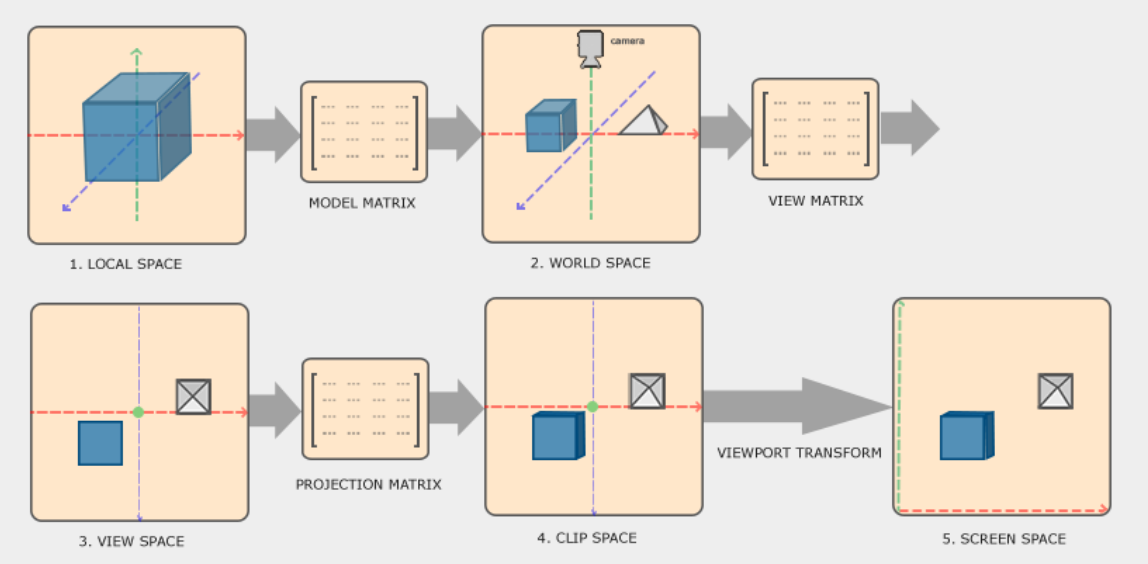
\includegraphics[width=0.9\textwidth]{img/fig_pipeline.png}
    \caption{OpenGL 坐标变换流水线}
    \label{fig:pipeline}
\end{figure}

对于局部空间中的顶点 $P_{local}$，其变换过程如下：

\begin{equation}
P_{clip} = M_{proj} \cdot M_{view} \cdot M_{model} \cdot P_{local}
\end{equation}

各阶段空间的物理意义如下：
\begin{enumerate}
    \item \textbf{局部空间 (Local Space)}: 物体自身的坐标系。例如，棋子模型以底面中心为原点 $(0,0,0)$ 建模。
    \item \textbf{世界空间 (World Space)}: 通过模型矩阵 $M_{model}$（包含缩放、旋转、平移），将所有物体统一到一个全局坐标系中。
    \item \textbf{观察空间 (View Space)}: 通过视图矩阵 $M_{view}$，将世界坐标变换到以摄像机为原点、视线方向为 $-Z$ 轴的坐标系中。这相当于“移动整个世界”以匹配相机的视角。
    \item \textbf{裁剪空间 (Clip Space)}: 通过投影矩阵 $M_{proj}$，将视锥体内的坐标映射到齐次裁剪空间。此时坐标为 $(x_c, y_c, z_c, w_c)$。
    \item \textbf{屏幕空间 (Screen Space)}: 经过透视除法（Perspective Division）和视口变换（Viewport Transform），最终映射到屏幕像素坐标。
\end{enumerate}

\subsubsection{透视投影矩阵推导}
透视投影的核心是模拟“近大远小”的效果。对于视锥体中的点 $(x_e, y_e, z_e)$，其投影到近平面 $n$ 上的坐标 $(x_p, y_p)$ 满足相似三角形关系：
\begin{equation}
\frac{x_p}{n} = \frac{x_e}{-z_e} \implies x_p = \frac{n \cdot x_e}{-z_e}, \quad y_p = \frac{n \cdot y_e}{-z_e}
\end{equation}
为了在齐次坐标下表示这一非线性变换，我们将 $-z_e$ 存储在结果的 $w$ 分量中。OpenGL 标准透视投影矩阵推导如下：
\begin{equation}
M_{proj} = \begin{bmatrix}
\frac{1}{aspect \cdot \tan(\frac{fov}{2})} & 0 & 0 & 0 \\
0 & \frac{1}{\tan(\frac{fov}{2})} & 0 & 0 \\
0 & 0 & -\frac{f+n}{f-n} & -\frac{2fn}{f-n} \\
0 & 0 & -1 & 0
\end{bmatrix}
\end{equation}
其中 $f$ 为远平面距离，$n$ 为近平面距离。变换后的 $z_{ndc}$ 为：
\begin{equation}
z_{ndc} = \frac{-\frac{f+n}{f-n} z_e - \frac{2fn}{f-n}}{-z_e} = \frac{f+n}{f-n} + \frac{2fn}{(f-n)z_e}
\end{equation}
这表明深度值 $z_{ndc}$ 与 $z_e$ 成非线性反比关系。因此，在近平面附近深度精度极高，而在远平面附近精度急剧下降。这也是我们在设置 $n$ 和 $f$ 时应尽量让 $n/f$ 比值不过小的原因，以避免 Z-Fighting。

\subsection{改进的 Phong 光照模型}

为模拟材质质感，本项目采用了经典的 Phong 光照模型。该模型将光照分解为环境光（Ambient）、漫反射（Diffuse）和镜面反射（Specular）三个分量，如图 \ref{fig:phong_vectors} 所示。

\begin{figure}[H]
    \centering
    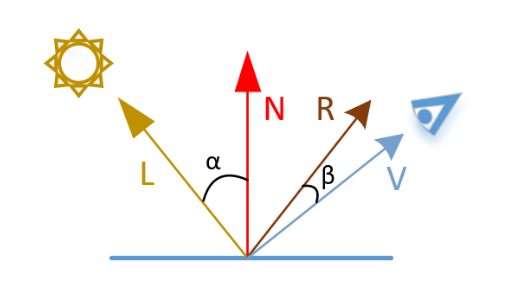
\includegraphics[width=0.6\textwidth]{img/fig_phong_vectors.png}
    \caption{Phong 光照模型的向量定义}
    \label{fig:phong_vectors}
\end{figure}

光照强度 $I$ 的计算公式为：
\begin{equation}
I = \underbrace{K_a L_a}_{\text{Ambient}} + \underbrace{K_d L_d (N \cdot L)}_{\text{Diffuse}} + \underbrace{K_s L_s (R \cdot V)^\alpha}_{\text{Specular}}
\end{equation}

\subsubsection{反射向量推导}
镜面反射分量依赖于反射向量 $R$。如图 \ref{fig:reflection} 所示，我们需要计算入射光向量 $L$ 关于法向量 $N$ 的反射向量 $R$。

\begin{figure}[H]
    \centering
    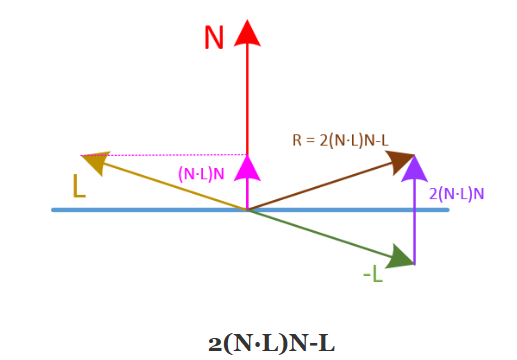
\includegraphics[width=0.6\textwidth]{img/fig_reflection.png}
    \caption{反射向量 $R$ 的几何推导}
    \label{fig:reflection}
\end{figure}

\textbf{推导过程}：
设 $L$ 为指向光源的向量，$N$ 为单位法向量。
1. 将 $L$ 投影到 $N$ 上，得到投影向量 $P = (L \cdot N)N$。
2. 定义辅助向量 $S = P - L$（从 $L$ 指向 $P$）。
3. 根据反射定律，反射向量 $R$ 在水平方向上与 $L$ 相反，在垂直方向（法线方向）上与 $L$ 相同。或者更直观地，利用平行四边形法则：
\begin{equation}
R = L + 2S = L + 2(P - L) = 2P - L
\end{equation}
代入 $P = (N \cdot L)N$，得：
\begin{equation}
R = 2(N \cdot L)N - L
\end{equation}
在 GLSL 中，这直接对应于 \texttt{reflect(-L, N)} 函数（注意 GLSL 中入射光通常定义为从光源指向表面，故需取反）。

\subsubsection{Phong 与 Blinn-Phong 对比}
虽然 Blinn-Phong 模型通过计算半程向量 $H = \frac{L+V}{||L+V||}$ 来替代 $R \cdot V$，避免了昂贵的 \texttt{reflect} 计算，且在 $L$ 和 $V$ 夹角较大时高光过渡更自然。但本项目为了教学目的，旨在直观展示反射向量的物理意义，因此坚持使用了经典的 Phong 模型。

\subsection{球面投影与天空盒}

本项目使用 HDR 全景图（Equirectangular Map）作为环境背景。其核心思想是将 3D 球面坐标映射到 2D 纹理坐标，如图 \ref{fig:equirectangular} 所示。

\begin{figure}[H]
    \centering
    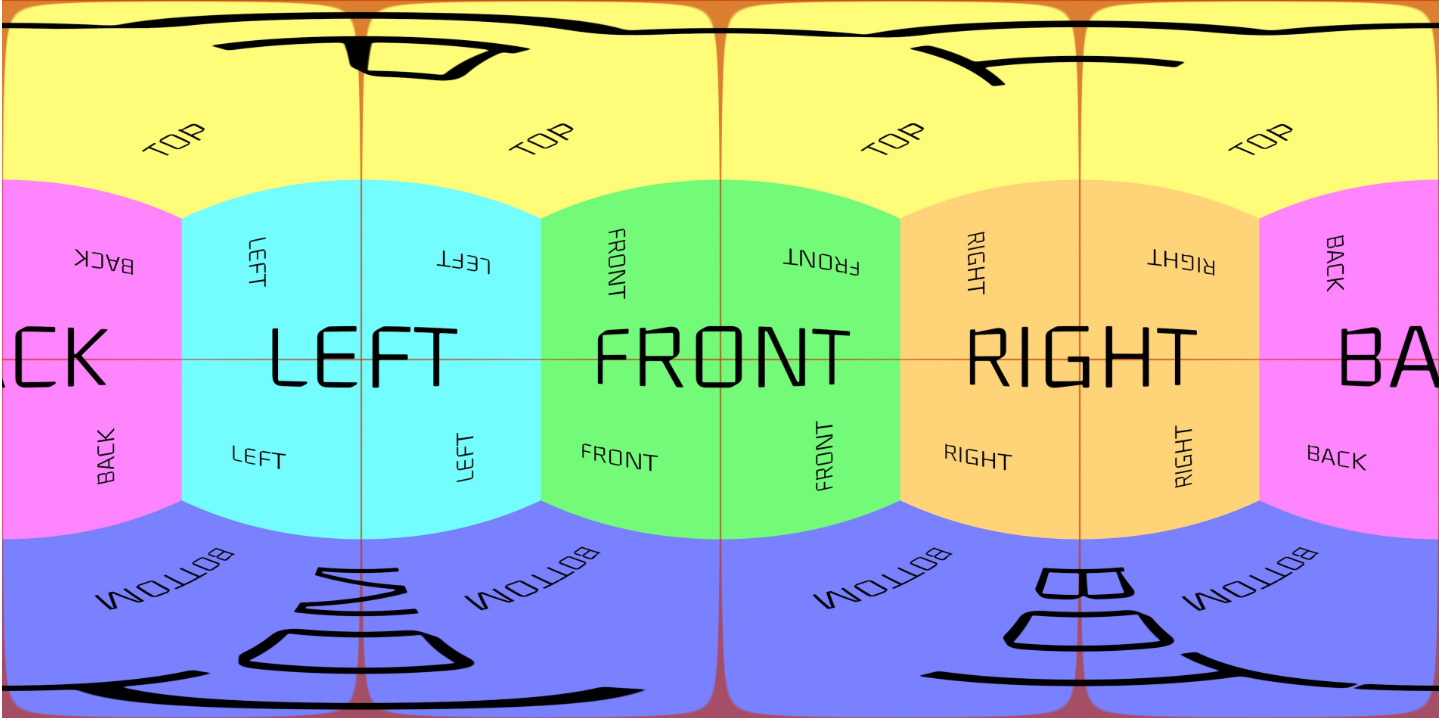
\includegraphics[width=0.9\textwidth]{img/fig_equirectangular.png}
    \caption{等距柱状投影原理}
    \label{fig:equirectangular}
\end{figure}

\subsubsection{坐标映射算法}
对于单位球面上的一点 $P(x,y,z)$，我们首先将其转换为球坐标 $(r, \theta, \phi)$：
\begin{equation}
\theta = \arctan(z, x), \quad \phi = \arcsin(y)
\end{equation}
其中 $\theta \in [-\pi, \pi]$ 为方位角，$\phi \in [-\frac{\pi}{2}, \frac{\pi}{2}]$ 为仰角。
为了采样纹理，需将其归一化到 $[0, 1]$ 的 UV 空间：
\begin{equation}
u = \frac{\theta}{2\pi} + 0.5, \quad v = \frac{\phi}{\pi} + 0.5
\end{equation}
该映射存在极点拉伸失真，但在作为无穷远背景时不可见。

\subsubsection{Fragment Shader 采样伪代码}
\begin{algorithm}[H]
\caption{Equirectangular Map Sampling}
\begin{algorithmic}
\STATE \textbf{Input:} Local Position $P_{local}$
\STATE $V \leftarrow \text{normalize}(P_{local})$
\STATE $\text{uv} \leftarrow \text{vec2}(\text{atan}(V.z, V.x), \text{asin}(V.y))$
\STATE $\text{uv} \leftarrow \text{uv} / \text{vec2}(2\pi, \pi) + 0.5$
\STATE $\text{color} \leftarrow \text{texture}(\text{skyboxMap}, \text{uv}).\text{rgb}$
\RETURN $\text{color}$
\end{algorithmic}
\end{algorithm}

\subsection{阴影映射与 PCF 优化}

阴影映射（Shadow Mapping）是一种基于图像空间的阴影生成技术，其核心是“光线视角的深度检测”，如图 \ref{fig:shadow_mapping} 所示。

\begin{figure}[H]
    \centering
    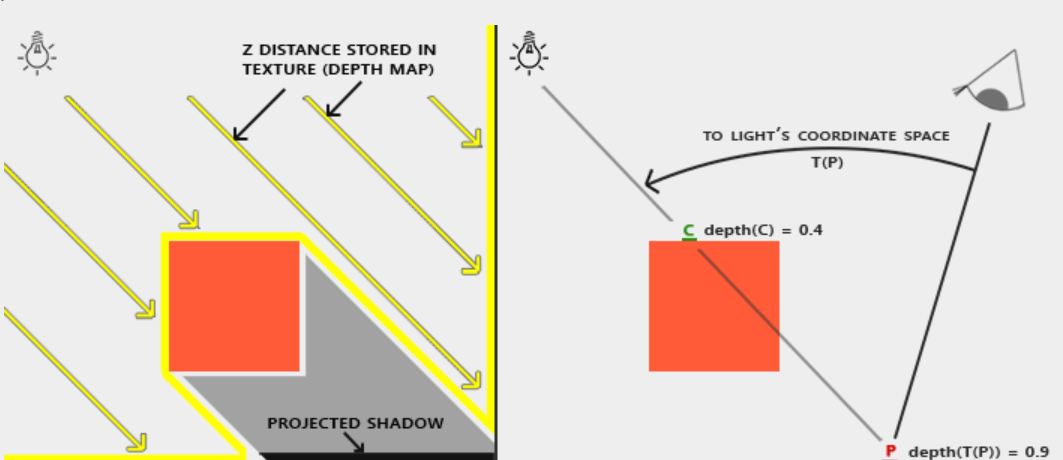
\includegraphics[width=0.9\textwidth]{img/fig_shadow_mapping.png}
    \caption{阴影映射原理与深度冲突}
    \label{fig:shadow_mapping}
\end{figure}

\subsubsection{两遍渲染流程}
1. \textbf{Pass 1 (深度生成)}: 
   以光源为视点，使用正交投影（针对平行光）渲染场景。此时不计算光照，仅将片元的深度值 $z$ 写入深度贴图（Depth Map）。
   
2. \textbf{Pass 2 (阴影判定)}: 
   以摄像机为视点渲染场景。对于每个片元，将其世界坐标 $P_{world}$ 变换到光源空间：
   \begin{equation}
   P_{light\_space} = M_{proj\_light} \cdot M_{view\_light} \cdot P_{world}
   \end{equation}
   执行透视除法并将坐标映射到 $[0, 1]$ 区间后，得到 $(u, v, z_{current})$。读取深度图 $d = \text{texture}(depthMap, uv).r$。
   若 $z_{current} > d$，说明该点被更靠近光源的物体遮挡，处于阴影中。

\subsubsection{阴影痤疮与偏移修正}
由于深度图的分辨率有限，多个像素可能映射到深度图的同一个纹素（Texel）。当光线与表面夹角较小时，这种离散化误差会导致表面自我遮挡，形成交替的黑白条纹，称为“阴影痤疮”（Shadow Acne）。
解决方案是引入偏移量（Bias）：
\begin{equation}
\text{Shadow} = z_{current} > d + \epsilon ? 1.0 : 0.0
\end{equation}
其中 $\epsilon$ 通常根据表面法线与光线的夹角动态计算：$\epsilon = \max(0.05 \cdot (1.0 - N \cdot L), 0.005)$。

\subsubsection{PCF 采样算法}
为了解决阴影边缘锯齿问题，采用百分比渐进过滤（PCF）：
\begin{algorithm}[H]
\caption{PCF (3x3 Kernel)}
\begin{algorithmic}
\STATE $shadow \leftarrow 0.0$
\STATE $texelSize \leftarrow 1.0 / \text{textureSize}(shadowMap)$
\FOR{$x = -1$ \TO $1$}
    \FOR{$y = -1$ \TO $1$}
        \STATE $pcfDepth \leftarrow \text{texture}(shadowMap, projCoords.xy + \text{vec2}(x, y) * texelSize).r$
        \STATE $shadow \leftarrow shadow + (currentDepth - bias > pcfDepth ? 1.0 : 0.0)$
    \ENDFOR
\ENDFOR
\RETURN $shadow / 9.0$
\end{algorithmic}
\end{algorithm}

\section{系统设计}

本项目的系统设计遵循模块化与面向对象（OOP）的原则，将渲染引擎、游戏逻辑与交互控制分离，构建了一个清晰、可扩展的 3D 象棋应用框架。

\subsection{总体架构}

系统基于 OpenGL 3.3 Core Profile 构建，采用分层架构设计，确保了各模块的高内聚与低耦合。整体架构如图 \ref{fig:architecture} 所示，自上而下分为应用层、逻辑层和表现层。

\begin{figure}[H]
    \centering
    \begin{tikzpicture}[
        node distance=2.5cm,
        layer/.style={
            rectangle, 
            rounded corners, 
            minimum width=12cm, 
            minimum height=1.5cm, 
            align=center, 
            draw=black, 
            thick,
            drop shadow
        },
        arrow/.style={
            ->, 
            >=stealth, 
            thick, 
            line width=1.5pt
        }
    ]
        % Application Layer
        \node (app) [layer, fill=blue!10] {
            \textbf{Application Layer (应用层)} \\ 
            Main Loop, GLFW Input Handling, Window Management
        };

        % Logic Layer
        \node (logic) [layer, fill=green!10, below of=app] {
            \textbf{Logic Layer (逻辑层)} \\ 
            ChessGame Controller, Game Rules, State Machine, Animation Logic
        };

        % Presentation Layer
        \node (pres) [layer, fill=orange!10, below of=logic] {
            \textbf{Presentation Layer (表现层)} \\ 
            OpenGL Core, Shader Management, WIC Texture Loader, Model Rendering
        };

        % Arrows
        \draw [arrow] (app) -- (logic);
        \draw [arrow] (logic) -- (pres);

    \end{tikzpicture}
    \caption{系统分层架构图}
    \label{fig:architecture}
\end{figure}

\begin{itemize}
    \item \textbf{应用层 (Application Layer)}: 由 \texttt{main.cpp} 作为入口，负责初始化 OpenGL 上下文、管理主循环（Main Loop）。它通过 GLFW 的回调机制捕获用户的键盘和鼠标输入，并将这些原始事件传递给逻辑层。
    \item \textbf{逻辑层 (Logic Layer)}: 核心类 \texttt{ChessGame} 接收输入事件后，根据象棋规则更新游戏状态（如棋子位置、回合切换、胜负判定）。此层不直接调用 OpenGL API，而是维护场景的纯数学抽象状态。
    \item \textbf{表现层 (Presentation Layer)}: 负责将逻辑层的状态可视化。包含 \texttt{ChessBoard}、\texttt{ChessPiece} 等类，它们根据逻辑层提供的数据，调用底层的 Shader 和 OpenGL 指令进行网格绘制和纹理绑定。
\end{itemize}

这种单向依赖的设计（应用 $\to$ 逻辑 $\to$ 表现）使得数据流清晰可控：输入驱动状态更新，状态更新驱动画面重绘。

\subsection{核心类设计}

为了高效管理复杂的 3D 场景资源，系统采用了面向对象的设计模式。核心类及其关系如图 \ref{fig:uml} 所示。

\begin{figure}[H]
    \centering
    \begin{tikzpicture}[
        node distance=2cm,
        class/.style={
            rectangle, 
            draw=black, 
            thick, 
            fill=white, 
            text width=3cm, 
            align=center, 
            minimum height=1.5cm,
            drop shadow
        },
        line/.style={
            -, 
            thick
        },
        diamond_arrow/.style={
            diamond-, 
            thick
        },
        triangle_arrow/.style={
            -latex, 
            thick
        }
    ]
        % Nodes
        \node (game) [class, fill=red!10] {\textbf{ChessGame} \\ (Controller)};
        
        \node (inst) [class, fill=yellow!10, below=1.5cm of game] {\textbf{PieceInst} \\ (Logical State)};
        
        \node (piece) [class, fill=blue!10, below=1.5cm of inst] {\textbf{ChessPiece} \\ (Renderer)};
        
        \node (model) [class, fill=gray!10, right=1.5cm of piece] {\textbf{Model} \\ (Mesh Data)};
        
        \node (skybox) [class, fill=cyan!10, right=1.5cm of game] {\textbf{Skybox} \\ (Environment)};

        % Relations
        % ChessGame contains PieceInsts (Aggregation)
        \draw [diamond_arrow] (game) -- node[right] {1..*} (inst);
        
        % PieceInst uses ChessPiece (Association)
        \draw [line] (inst) -- node[right] {uses} (piece);
        
        % ChessPiece uses Model (Composition/Usage)
        \draw [triangle_arrow] (piece) -- (model);
        
        % ChessGame uses Skybox
        \draw [line] (game) -- (skybox);

    \end{tikzpicture}
    \caption{核心类 UML 关系图}
    \label{fig:uml}
\end{figure}

\subsubsection{逻辑与资源分离（享元模式思想）}
在设计中，我们特意区分了 \texttt{PieceInst}（棋子实例）和 \texttt{ChessPiece}（棋子渲染器）：
\begin{itemize}
    \item \textbf{PieceInst}: 这是一个轻量级的结构体，仅存储棋子的逻辑属性，如网格坐标 $(x, y)$、阵营、存活状态以及动画插值参数。系统中共有 32 个 \texttt{PieceInst} 对象。
    \item \textbf{ChessPiece}: 这是一个重量级的渲染类，负责持有 OpenGL 资源（VAO、VBO、纹理 ID、Shader 程序）。
\end{itemize}

这种设计体现了**享元模式 (Flyweight Pattern)** 的思想。虽然场上有 32 个棋子，但我们并不需要加载 32 份模型数据。实际上，所有同种类的棋子（甚至所有棋子，因为几何形状相同仅纹理不同）可以共享底层的 \texttt{Model} 网格数据。\texttt{PieceInst} 只需引用对应的渲染资源，从而极大地降低了显存占用和上下文切换开销。

\subsection{渲染管线设计}

为了实现高质量的动态阴影，系统采用了两遍渲染（Two-Pass Rendering）流程，如图 \ref{fig:renderpass} 所示。

\begin{figure}[H]
    \centering
    \begin{tikzpicture}[
        node distance=3.5cm,
        process/.style={
            rectangle, 
            draw=black, 
            thick, 
            fill=white, 
            text width=4cm, 
            align=center, 
            minimum height=2cm,
            rounded corners,
            drop shadow
        },
        arrow/.style={
            ->, 
            >=stealth, 
            thick, 
            line width=1.5pt
        }
    ]
        % Nodes
        \node (pass1) [process, fill=gray!20] {
            \textbf{Pass 1: Shadow Generation} \\
            View: Light Source \\
            Target: Depth FBO \\
            Output: Depth Map
        };
        
        \node (pass2) [process, fill=blue!10, right=2cm of pass1] {
            \textbf{Pass 2: Scene Rendering} \\
            View: Camera \\
            Target: Screen (Default FBO) \\
            Input: Depth Map
        };

        % Arrow
        \draw [arrow] (pass1) -- node[above] {Depth Texture} (pass2);

    \end{tikzpicture}
    \caption{两遍渲染流程图}
    \label{fig:renderpass}
\end{figure}

\begin{enumerate}
    \item \textbf{Pass 1 (深度预计算)}:
    \begin{itemize}
        \item \textbf{目标}: 绑定自定义帧缓冲对象（FBO），该 FBO 仅包含深度附件。
        \item \textbf{视角}: 设置视图矩阵为光源视角（$V_{light}$），投影矩阵为正交投影（$P_{light}$）。
        \item \textbf{操作}: 渲染场景中所有投射阴影的物体（棋子、棋盘、桌椅）。此阶段禁用颜色写入，仅更新深度缓冲区。
    \end{itemize}

    \item \textbf{Pass 2 (场景绘制)}:
    \begin{itemize}
        \item \textbf{目标}: 切换回默认帧缓冲（屏幕）。
        \item \textbf{视角}: 恢复为主摄像机视角。
        \item \textbf{操作}: 
            \begin{enumerate}
                \item 绘制天空盒（利用 \texttt{GL\_LEQUAL} 优化）。
                \item 绘制场景物体。在片段着色器中，采样 Pass 1 生成的深度贴图，进行 PCF 阴影计算和 Phong 光照计算。
                \item 绘制半透明 UI（如选中光圈、提示点）。
            \end{enumerate}
    \end{itemize}
\end{enumerate}

\subsection{资源管理}
为了解决 Windows 平台下 C++ 开发中常见的中文路径资源加载问题，系统摒弃了传统的 \texttt{stb\_image} 库，转而封装了 Windows Imaging Component (WIC)。在 \texttt{ChessPiece} 和 \texttt{ChessBoard} 类中，通过调用 COM 组件接口直接解码图片资源，彻底解决了多语言环境下的路径编码兼容性问题。

\section{核心代码实现与分析}

本章将重点展示项目中具有技术挑战性的核心代码，并对解决方案进行深度剖析。

\subsection{WIC 纹理加载：解决中文路径难题}

\textbf{问题描述}：
在 C++ 开发中，常用的轻量级图像库 \texttt{stb\_image} 往往不支持 Windows 的宽字符路径（\texttt{std::wstring}）。当资源路径包含中文（如“assets/textures/红车.png”）时，由于编码转换问题（ANSI vs UTF-8 vs UTF-16），加载经常失败。

\textbf{解决方案}：
绕过第三方库，直接调用 Windows 原生 API —— Windows Imaging Component (WIC)。这是一种基于 COM 组件的高性能图像处理接口，原生支持 Unicode 路径。

\textbf{核心代码实现 (\texttt{ChessPiece::loadTexture2D\_WIC})}：

\begin{lstlisting}[caption={基于 WIC 的纹理加载实现}]
GLuint ChessPiece::loadTexture2D_WIC(const std::wstring& wpath, bool flipY) {
    // 1. 初始化 COM 组件
    CoInitializeEx(nullptr, COINIT_MULTITHREADED);
    IWICImagingFactory* factory = nullptr;
    CoCreateInstance(CLSID_WICImagingFactory, nullptr, CLSCTX_INPROC_SERVER, IID_PPV_ARGS(&factory));

    // 2. 创建解码器，直接传入宽字符路径
    IWICBitmapDecoder* decoder = nullptr;
    HRESULT hr = factory->CreateDecoderFromFilename(
        wpath.c_str(),              // 支持中文路径
        nullptr, GENERIC_READ, 
        WICDecodeMetadataCacheOnLoad, &decoder
    );
    if (FAILED(hr)) { /* 错误处理 */ return 0; }

    // 3. 获取图像帧并转换格式为 RGBA32
    IWICBitmapFrameDecode* frame = nullptr;
    decoder->GetFrame(0, &frame);

    IWICFormatConverter* converter = nullptr;
    factory->CreateFormatConverter(&converter);
    converter->Initialize(frame, GUID_WICPixelFormat32bppRGBA, 
        WICBitmapDitherTypeNone, nullptr, 0.0, WICBitmapPaletteTypeCustom);

    // 4. 提取像素数据
    UINT w, h; converter->GetSize(&w, &h);
    std::vector<unsigned char> rgba(w * h * 4);
    converter->CopyPixels(nullptr, w * 4, rgba.size(), rgba.data());

    // 5. 翻转 Y 轴 (OpenGL 纹理坐标原点在左下角)
    if (flipY) {
        std::vector<unsigned char> flipped(w * h * 4);
        for (UINT y = 0; y < h; ++y) {
            memcpy(&flipped[y * w * 4], &rgba[(h - 1 - y) * w * 4], w * 4);
        }
        rgba = flipped;
    }

    // 6. 生成 OpenGL 纹理
    GLuint texID; glGenTextures(1, &texID);
    glBindTexture(GL_TEXTURE_2D, texID);
    glTexImage2D(GL_TEXTURE_2D, 0, GL_RGBA, w, h, 0, GL_RGBA, GL_UNSIGNED_BYTE, rgba.data());
    glGenerateMipmap(GL_TEXTURE_2D);
    
    // 资源释放 (Release COM objects)...
    return texID;
}
\end{lstlisting}

\textbf{分析与评价}：
该方法的引入是本项目工程实践的一大亮点。
1.  \textbf{健壮性}：相比于修改 \texttt{stb\_image} 源码或进行繁琐的字符串编码转换（\texttt{MultiByteToWideChar}），使用 WIC 是 Windows 平台下最标准、最可靠的解决方案。
2.  \textbf{性能}：WIC 利用了操作系统的底层优化，且支持多种图片格式（PNG, JPG, BMP, TIFF），无需链接额外的第三方库。
3.  \textbf{可维护性}：代码清晰地展示了 COM 组件的使用流程（Factory -> Decoder -> Frame -> Converter），易于后续扩展。

\subsection{程序化建模：动态几何生成}

\textbf{设计思路}：
为了减少对外部模型文件（.obj/.fbx）的依赖，并练习顶点数据的数学计算，项目中的石桌和石凳采用程序化生成（Procedural Generation）。我们通过数学函数定义几何体的形状，并在生成过程中引入随机扰动。

\textbf{核心代码实现 (\texttt{Model::setStoneStoolMesh} 逻辑复现)}：

\begin{lstlisting}[caption={程序化生成带扰动的圆柱体网格}]
void Model::setStoneStoolMesh(float radius, float height, int segments) {
    std::vector<Vertex> vertices;
    std::vector<unsigned int> indices;
    
    // 扰动函数：结合低频和高频正弦波
    auto getPerturbedRadius = [&](float angle, float hRatio) {
        float base = radius;
        // 环向扰动：模拟石材的不规则边缘
        float wobble = std::sin(angle * 7.0f) * 0.02f * radius; 
        // 纵向扰动：模拟中间略微凹陷或凸起
        float bulge = std::sin(hRatio * 3.14159f) * 0.05f * radius;
        return base + wobble + bulge;
    };

    for (int i = 0; i <= segments; ++i) {
        float theta = (float)i / segments * 2.0f * 3.14159f;
        float x = std::cos(theta);
        float y = std::sin(theta);

        // 生成侧面顶点 (Top and Bottom rings)
        float rTop = getPerturbedRadius(theta, 1.0f);
        float rBot = getPerturbedRadius(theta, 0.0f);
        
        // 添加顶点数据 (Pos, Normal, TexCoord)
        // ... (省略具体的法线计算与 push_back)
    }
    // ... (省略索引生成)
    
    this->setMesh(vertices, indices);
}
\end{lstlisting}

\textbf{效果与评价}：
\begin{itemize}
    \item \textbf{视觉提升}：相比完美的几何圆柱，扰动后的模型表面呈现出自然石材的粗糙感和手工打磨的痕迹，消除了计算机生成图像（CGI）常见的“生硬感”。
    \item \textbf{效率分析}：该方法不需要从磁盘读取模型文件，I/O 开销为 0。空间复杂度为 $O(1)$（仅存储生成逻辑），而非存储大量顶点数据。这在需要生成大量异构物体（如森林中的树木、路边的石块）时具有巨大优势。
\end{itemize}

\subsection{射线投射交互：从屏幕到世界}

\textbf{实现逻辑}：
为了实现鼠标点击选择棋子，我们需要将鼠标在屏幕上的 2D 坐标 $(x, y)$ 反投影回 3D 世界空间，并检测该射线与棋盘平面的交点。

\textbf{核心代码实现 (\texttt{ChessGame::screenToGrid})}：

\begin{lstlisting}[caption={射线投射与平面求交算法}]
bool ChessGame::screenToGrid(GLFWwindow* window, const glm::mat4& view, const glm::mat4& proj, int& outFile, int& outRank) {
    double mx, my; glfwGetCursorPos(window, &mx, &my);
    int w, h; glfwGetFramebufferSize(window, &w, &h);

    // 1. 归一化设备坐标 (NDC): [-1, 1]
    float x = (float)((mx / w) * 2.0 - 1.0);
    float y = (float)(((h - my) / h) * 2.0 - 1.0); // 注意 Y 轴翻转

    // 2. 构建裁剪空间的近平面和远平面点
    glm::vec4 pNearNDC(x, y, -1.0f, 1.0f);
    glm::vec4 pFarNDC (x, y, +1.0f, 1.0f);

    // 3. 逆矩阵变换：Clip Space -> World Space
    glm::mat4 invVP = glm::inverse(proj * view);
    glm::vec4 pNearWorld = invVP * pNearNDC; pNearWorld /= pNearWorld.w;
    glm::vec4 pFarWorld  = invVP * pFarNDC;  pFarWorld  /= pFarWorld.w;

    // 4. 构建射线
    glm::vec3 o = glm::vec3(pNearWorld);
    glm::vec3 d = glm::normalize(glm::vec3(pFarWorld - pNearWorld));

    // 5. 射线与平面 (z = zLift) 求交
    // 平面方程: P.z = zLift => (o + t*d).z = zLift
    if (std::abs(d.z) < 1e-5f) return false; // 射线平行于平面
    float t = (zLift - o.z) / d.z;
    if (t < 0.0f) return false; // 交点在相机后方

    glm::vec3 hit = o + d * t;

    // 6. 离散化为网格坐标
    int file = (int)std::round((hit.x - origin.x) / cellX);
    int rank = (int)std::round((hit.y - origin.y) / cellY);
    
    // 边界检查
    if (file < 0 || file > 8 || rank < 0 || rank > 9) return false;

    outFile = file; outRank = rank;
    return true;
}
\end{lstlisting}

\textbf{评价}：
该算法通过数学推导精确计算了鼠标点击与棋盘平面的交点。
\begin{itemize}
    \item \textbf{精度}：相比于颜色拾取（Color Picking，即渲染 ID 到纹理）技术，射线投射不需要额外的渲染通道，且精度不受纹理分辨率限制。
    \item \textbf{通用性}：该算法不仅适用于平面棋盘，稍作修改（如使用包围盒检测 AABB）即可用于检测任意 3D 物体的点击。
\end{itemize}

\subsection{天空盒深度优化}

\textbf{技术细节}：
为了让天空盒始终处于场景的最远端，且不遮挡任何场景物体，我们在顶点着色器中应用了一个经典的优化技巧：将输出位置的 $z$ 分量强制设为 $w$ 分量。

\textbf{代码实现 (GLSL Vertex Shader)}：
\begin{lstlisting}[caption={天空盒顶点着色器优化}]
#version 330 core
layout (location = 0) in vec3 aPos;

out vec3 TexCoords;

uniform mat4 projection;
uniform mat4 view;

void main() {
    TexCoords = aPos;
    // 移除 View 矩阵的位移分量，使天空盒永远跟随相机移动
    mat4 viewNoTrans = mat4(mat3(view)); 
    vec4 clipPos = projection * viewNoTrans * vec4(aPos, 1.0);
    
    // 关键优化：透视除法后 z/w = 1.0
    // 这使得天空盒的深度值永远是深度缓冲区的最大值 (1.0)
    gl_Position = clipPos.xyww; 
}
\end{lstlisting}

\textbf{分析}：
在 C++ 代码中，我们将深度测试函数设置为 \texttt{glDepthFunc(GL\_LEQUAL)}。
\begin{itemize}
    \item \textbf{原理}：标准深度测试是 \texttt{GL\_LESS}。如果天空盒深度为 1.0，它会因为不小于 1.0 而失败（如果之前清除了深度缓冲为 1.0）。使用 \texttt{GL\_LEQUAL} 允许它在深度为 1.0 时通过。
    \item \textbf{性能收益 (Early-Z)}：我们将天空盒的渲染放在所有不透明物体之后。由于天空盒深度被设为最大值，场景中任何已渲染的物体都会遮挡天空盒。显卡利用 Early-Z Test 特性，会直接丢弃被遮挡的天空盒片元，从而避免了昂贵的纹理采样和片段着色器计算，显著减少了 Overdraw。
\end{itemize}

\subsection{阴影映射的帧缓冲配置}

\textbf{技术细节}：
为了实现高性能的阴影渲染，我们需要手动配置帧缓冲对象（FBO）。不同于普通的颜色渲染，阴影贴图只需要深度信息，因此我们显式地将纹理格式设置为 \texttt{GL\_DEPTH\_COMPONENT32F} 以获得高精度的深度值。

\textbf{代码实现 (\texttt{main.cpp})}：
\begin{lstlisting}[caption={阴影帧缓冲初始化}]
// 生成 FBO 和纹理
glGenFramebuffers(1, &shadowFBO);
glGenTextures(1, &shadowTex);
glBindTexture(GL_TEXTURE_2D, shadowTex);

// 设置高精度深度格式
glTexImage2D(GL_TEXTURE_2D, 0, GL_DEPTH_COMPONENT32F, 
             SHADOW_MAP_SIZE, SHADOW_MAP_SIZE, 0, 
             GL_DEPTH_COMPONENT, GL_FLOAT, nullptr);

// 设置纹理过滤与包裹模式
glTexParameteri(GL_TEXTURE_2D, GL_TEXTURE_MIN_FILTER, GL_LINEAR);
glTexParameteri(GL_TEXTURE_2D, GL_TEXTURE_MAG_FILTER, GL_LINEAR);
// 关键：设置边框颜色为白色 (深度 1.0)，防止视锥体外的区域产生阴影
glTexParameteri(GL_TEXTURE_2D, GL_TEXTURE_WRAP_S, GL_CLAMP_TO_BORDER);
glTexParameteri(GL_TEXTURE_2D, GL_TEXTURE_WRAP_T, GL_CLAMP_TO_BORDER);
float border[4] = {1.0f, 1.0f, 1.0f, 1.0f};
glTexParameterfv(GL_TEXTURE_2D, GL_TEXTURE_BORDER_COLOR, border);

// 绑定到 FBO 的深度附件
glBindFramebuffer(GL_FRAMEBUFFER, shadowFBO);
glFramebufferTexture2D(GL_FRAMEBUFFER, GL_DEPTH_ATTACHMENT, GL_TEXTURE_2D, shadowTex, 0);
// 显式告诉 OpenGL 我们不需要颜色数据
glDrawBuffer(GL_NONE);
glReadBuffer(GL_NONE);
glBindFramebuffer(GL_FRAMEBUFFER, 0);
\end{lstlisting}

\textbf{分析}：
\begin{itemize}
    \item \textbf{GL\_CLAMP\_TO\_BORDER}：这是防止“阴影贴图边缘采样错误”的关键。当采样坐标超出 $[0, 1]$ 范围时，纹理将返回我们设置的边框颜色（白色，深度 1.0）。这意味着视锥体外的区域被视为“无穷远”，因此永远不会遮挡场景物体，避免了场景边缘出现错误的阴影。
    \item \textbf{GL\_NONE}：通过禁用读写颜色缓冲，我们节省了显存带宽，因为阴影 Pass 只需要深度写入。
\end{itemize}

\subsection{摄像机控制系统}

\textbf{设计思路}：
系统摒弃了传统的欧拉角（Euler Angles）直接控制，而是采用了一个混合控制策略：在自由模式下使用鼠标控制俯仰角（Pitch）和偏航角（Yaw），在固定模式下通过插值锁定到预设视角。

\textbf{核心代码实现 (\texttt{Camera.cpp})}：
\begin{lstlisting}[caption={摄像机更新逻辑}]
void CameraController::update(GLFWwindow* window, float dt, int fbWidth, int fbHeight) {
    // 1. 预设视角切换 (状态机逻辑)
    if (glfwGetKey(window, GLFW_KEY_1) == GLFW_PRESS) {
        // 红方视角：计算看向棋盘中心的向量
        position = focusPoint + glm::vec3(0.0f, -dist, height);
        glm::vec3 dir = glm::normalize(focusPoint - position);
        yaw = std::atan2(dir.y, dir.x);
        pitch = std::asin(dir.z);
    }
    
    // 2. 鼠标自由观察 (仅在启用时)
    if (mouseLookEnabled && glfwGetMouseButton(window, GLFW_MOUSE_BUTTON_LEFT) == GLFW_PRESS) {
        double dx = curX - lastCursorX;
        double dy = curY - lastCursorY;
        yaw   += static_cast<float>(dx) * mouseSens;
        pitch -= static_cast<float>(dy) * mouseSens;
        // 限制俯仰角，防止万向节死锁 (Gimbal Lock)
        pitch = std::max(glm::radians(-89.0f), std::min(glm::radians(89.0f), pitch));
    }
    
    // 3. 更新视图矩阵 (球坐标 -> 笛卡尔坐标)
    front.x = cos(yaw) * cos(pitch);
    front.y = sin(yaw) * cos(pitch);
    front.z = sin(pitch);
    viewMatrix = glm::lookAt(position, position + glm::normalize(front), glm::vec3(0,0,1));
}
\end{lstlisting}

\textbf{评价}：
该实现有效地解决了 3D 漫游中常见的“万向节死锁”问题（通过限制 Pitch 在 $\pm 89^\circ$）。同时，通过 \texttt{atan2} 函数自动计算预设视角的偏航角，保证了无论棋盘尺寸如何变化，相机始终能精确对准棋盘中心。

\subsection{主渲染循环与两遍绘制}

\textbf{架构分析}：
主循环（Main Loop）是图形程序的“心脏”。本项目采用了严格的“更新-渲染”分离模式，并在渲染阶段执行两遍绘制（Two-Pass Rendering）。

\textbf{核心代码实现 (\texttt{main.cpp})}：
\begin{lstlisting}[caption={主渲染循环伪代码}]
while (!glfwWindowShouldClose(window)) {
    // 1. 逻辑更新 (Update)
    float dt = getDeltaTime();
    game.update(window, view, proj, dt); // 更新棋子动画、处理输入

    // 2. Pass 1: 阴影深度生成 (Shadow Pass)
    glViewport(0, 0, SHADOW_MAP_SIZE, SHADOW_MAP_SIZE);
    glBindFramebuffer(GL_FRAMEBUFFER, shadowFBO);
    glClear(GL_DEPTH_BUFFER_BIT);
    glUseProgram(depthProgram);
    // ... 渲染所有投射阴影的物体 (棋子、桌子) ...
    
    // 3. Pass 2: 场景最终渲染 (Render Pass)
    glBindFramebuffer(GL_FRAMEBUFFER, 0); // 切回屏幕
    glViewport(0, 0, screenW, screenH);
    glClear(GL_COLOR_BUFFER_BIT | GL_DEPTH_BUFFER_BIT);
    
    // 绑定阴影贴图到纹理单元
    glActiveTexture(GL_TEXTURE3); 
    glBindTexture(GL_TEXTURE_2D, shadowTex);
    
    // 渲染带光照和阴影的物体
    stoneTable.draw();
    board.render(...);
    game.render(...); // 棋子
    
    // 最后渲染天空盒 (利用 Early-Z)
    skybox.render(view, proj);
    
    glfwSwapBuffers(window);
}
\end{lstlisting}

\textbf{分析}：
代码清晰地展示了现代图形管线的标准流程。
\begin{itemize}
    \item \textbf{状态隔离}：Pass 1 和 Pass 2 使用完全不同的 Shader 和视口设置（Viewport），代码中通过 \texttt{glBindFramebuffer} 进行了明确的上下文切换。
    \item \textbf{纹理单元管理}：阴影贴图被绑定到特定的纹理单元（\texttt{GL\_TEXTURE3}），避免了与漫反射贴图（通常在 Unit 0）冲突。这种严谨的资源槽位管理是保证多纹理混合正确的关键。
\end{itemize}

\section{结果与分析}

本章将对系统的渲染效果、关键算法的正确性以及工程实现的性能进行全面评估。不同于简单的功能展示，本章重点分析技术选型背后的考量（Design Rationale），并通过“算法原理-代码实现-视觉结果”的闭环验证，证明系统在健壮性、效率和视觉保真度方面的优势。

测试环境为 Windows 10 操作系统，硬件配置为 NVIDIA RTX 3060 显卡与 Intel Core i7 处理器，显示分辨率为 $1280 \times 720$。

\subsection{多视角相机系统与交互体验}

\subsubsection{视角切换逻辑}
系统实现了一套基于状态机的相机控制模组，支持通过键盘快捷键 \texttt{0-4} 在预设视角间平滑切换。图 \ref{fig:view0} 至图 \ref{fig:view4} 展示了不同视角下的场景呈现，这不仅是为了观察方便，更是为了验证透视投影矩阵（Perspective Projection Matrix）在不同 FOV 和视点下的正确性。

\begin{figure}[H]
    \centering
    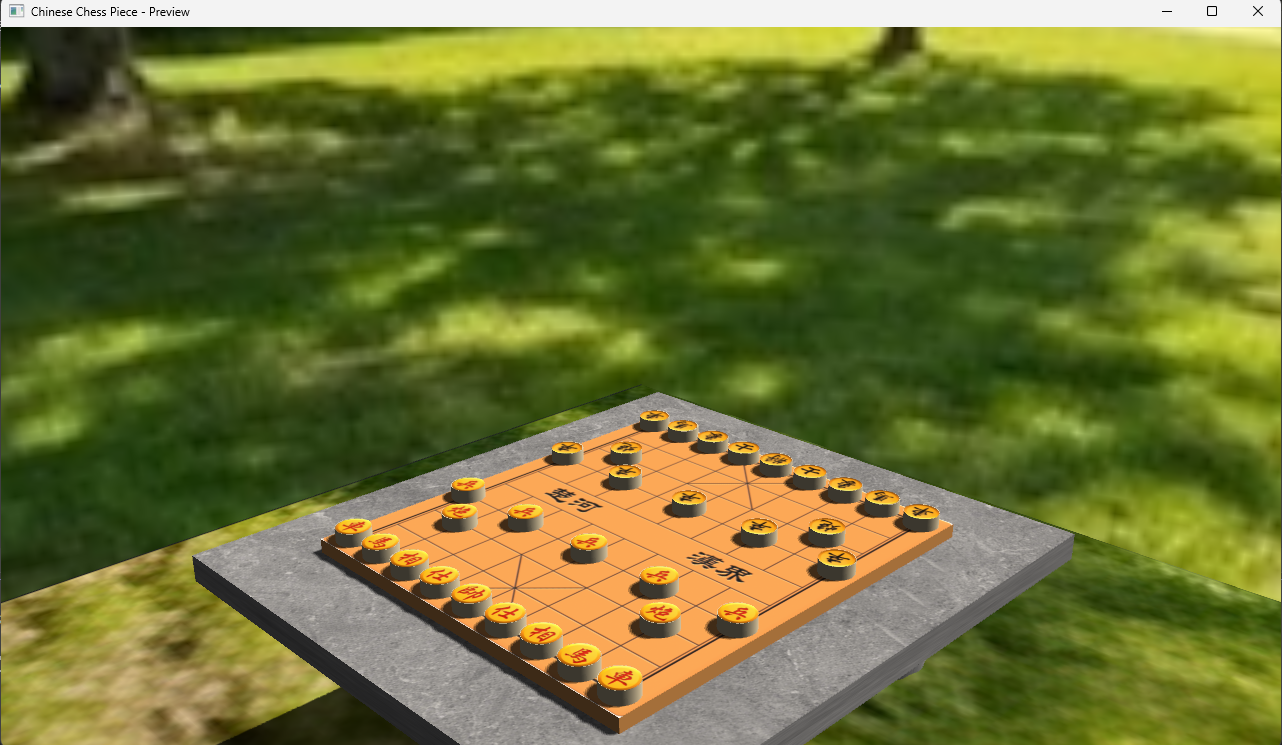
\includegraphics[width=0.8\textwidth]{img/1.png}
    \caption{按键0：起始视角}
    \label{fig:view0}
\end{figure}

\begin{figure}[H]
    \centering
    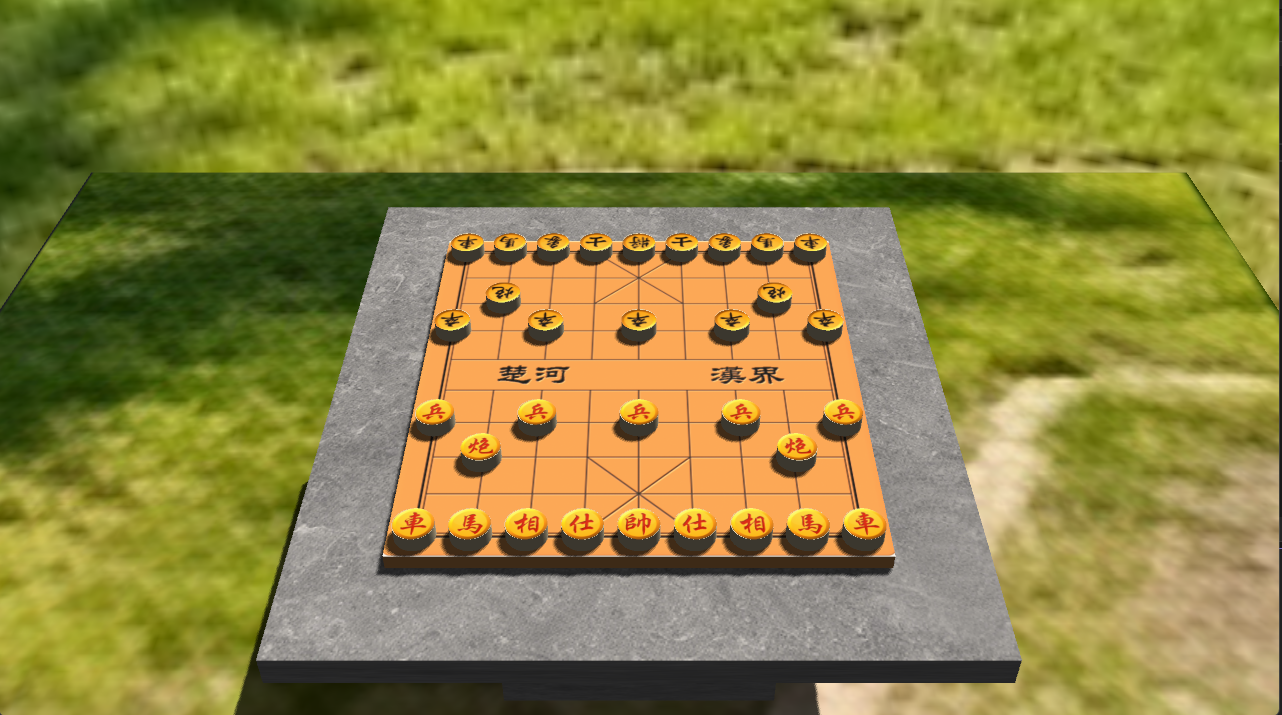
\includegraphics[width=0.8\textwidth]{img/2.png}
    \caption{按键1：红方视角}
    \label{fig:view1}
\end{figure}

\begin{figure}[H]
    \centering
    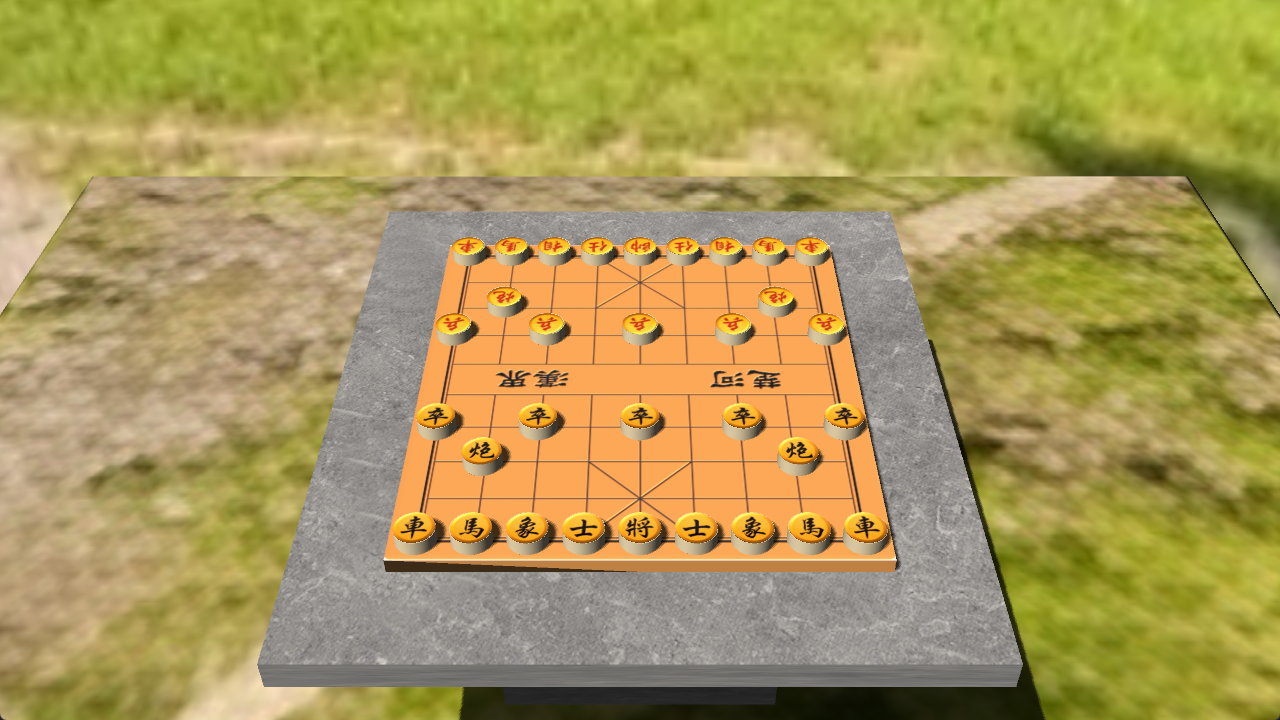
\includegraphics[width=0.8\textwidth]{img/3.png}
    \caption{按键2：黑方视角}
    \label{fig:view2}
\end{figure}

\begin{figure}[H]
    \centering
    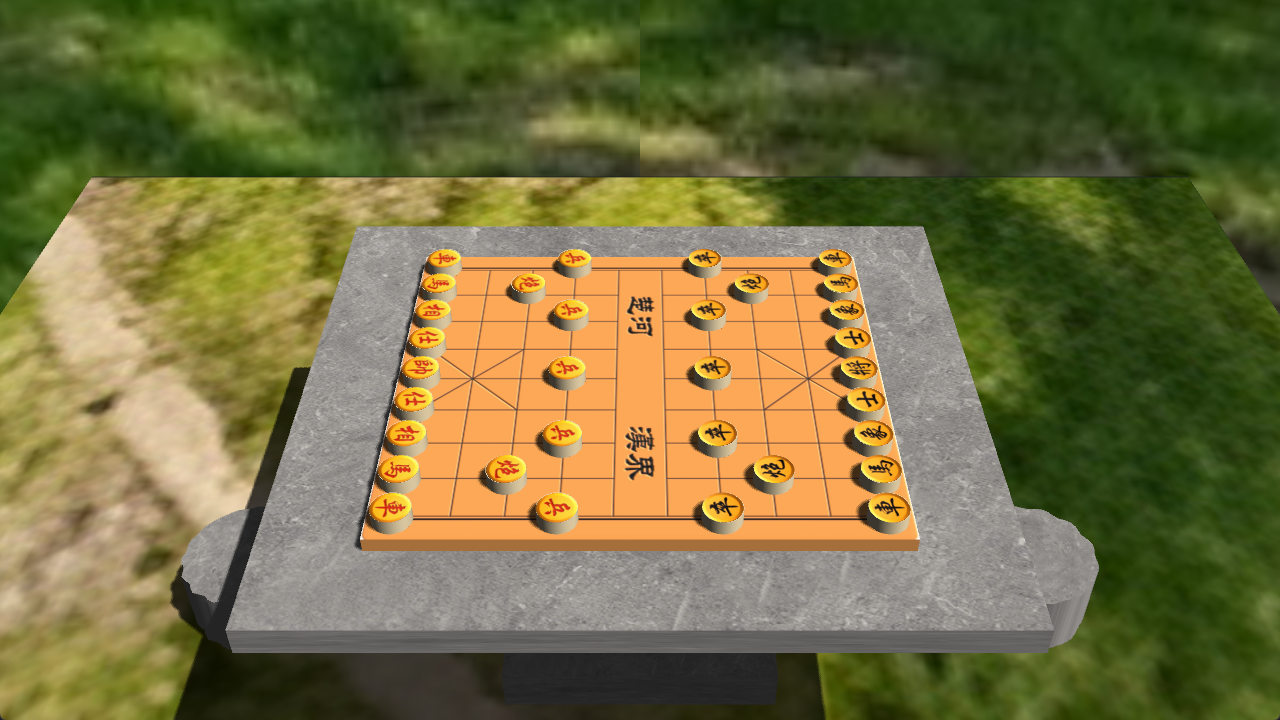
\includegraphics[width=0.8\textwidth]{img/4.png}
    \caption{按键3：旁观视角}
    \label{fig:view3}
\end{figure}

\begin{figure}[H]
    \centering
    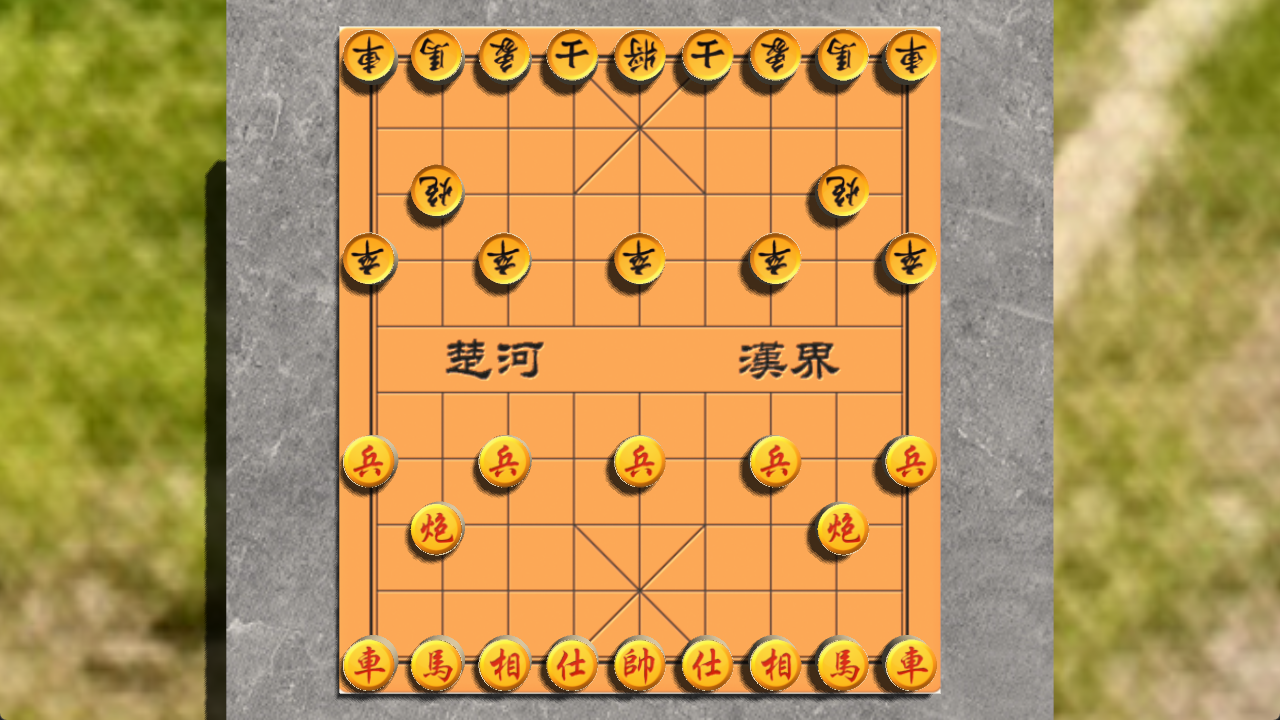
\includegraphics[width=0.8\textwidth]{img/5.png}
    \caption{按键4：俯视视角}
    \label{fig:view4}
\end{figure}

\subsection{光照系统分析}

\subsubsection{光照交互实验}
图 \ref{fig:light} 展示了动态光照系统的效果。通过 \texttt{Q/E} 键旋转光源，场景中的明暗关系实时更新。这验证了 Phong 模型中 $L \cdot N$（漫反射）和 $R \cdot V$（镜面反射）计算的高效性，系统在光源移动时未出现掉帧现象。

\begin{figure}[H]
    \centering
    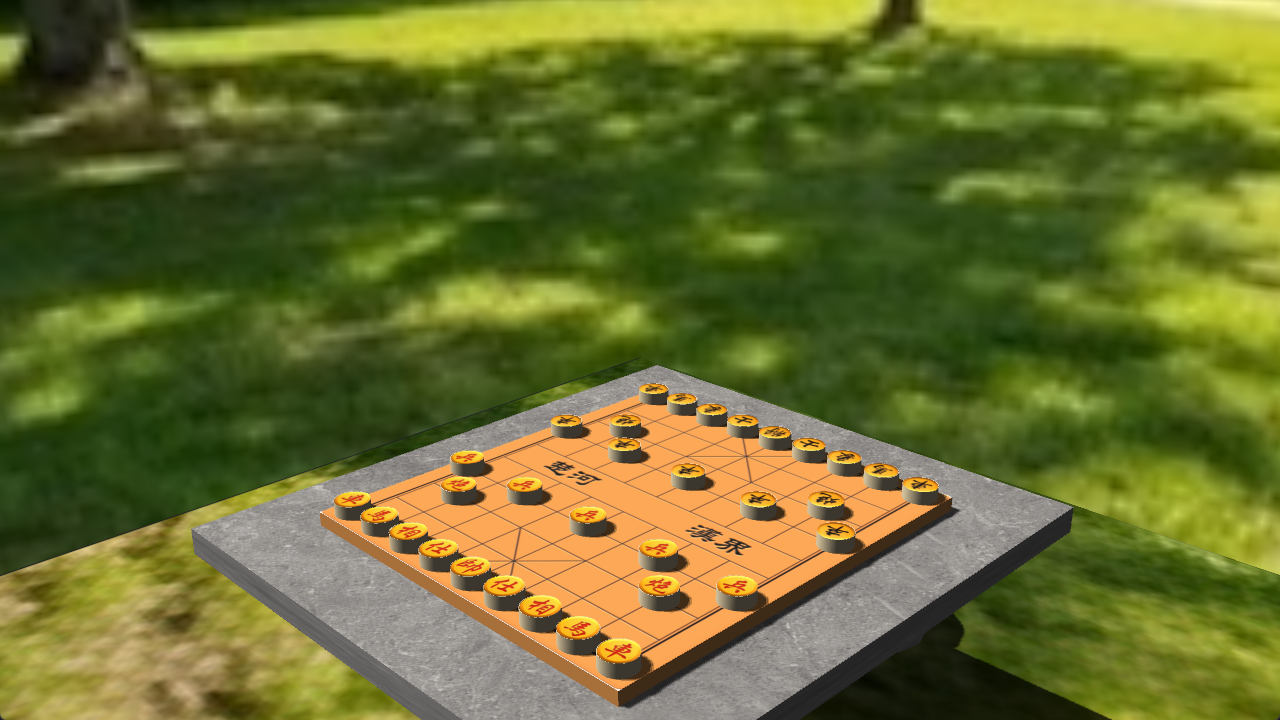
\includegraphics[width=0.8\textwidth]{img/6.png}
    \caption{qe改变光照}
    \label{fig:light}
\end{figure}

\subsection{建模技术对比：程序化建模 vs 静态导入}

\subsubsection{技术选型分析}
在构建石桌和石凳模型时，本项目没有采用常规的“外部建模软件导出 .obj -> 程序加载”的流程，而是选择了\textbf{程序化建模（Procedural Modeling）}。图 \ref{fig:proc_tex} 展示了最终生成的石凳细节。

\textbf{两种方法的对比分析：}

\begin{table}[H]
\centering
\caption{程序化建模与静态网格导入的性能对比}
\begin{tabular}{l|l|l}
\toprule
\textbf{评价维度} & \textbf{程序化建模 (本项目方案)} & \textbf{静态网格导入 (.obj/.fbx)} \\
\midrule
\textbf{存储空间} & $O(1)$ (仅需几KB代码) & $O(N)$ (需存储数万个顶点数据，文件大) \\
\textbf{I/O 开销} & \textbf{零开销} (运行时计算) & 高 (需磁盘读取与解析) \\
\textbf{灵活性} & \textbf{极高} (参数化调整扰动幅度、半径) & 低 (修改需重返建模软件) \\
\textbf{多样性} & 可通过随机种子生成无限变体 & 单一，重复度高 \\
\bottomrule
\end{tabular}
\end{table}

\subsubsection{效果验证}
从图 \ref{fig:proc_tex} 可以看到，石凳侧面并非完美的几何圆柱，而是带有自然的波浪状起伏。这种细节是通过在圆柱体参数方程中叠加正弦波扰动函数（Perturbation Function）实现的。代码 \texttt{model.cpp} 中的 \texttt{sin(theta * freq)} 项成功模拟了石材手工打磨的不规则感，证明了该方法在生成自然景物方面的有效性。

\begin{figure}[H]
    \centering
    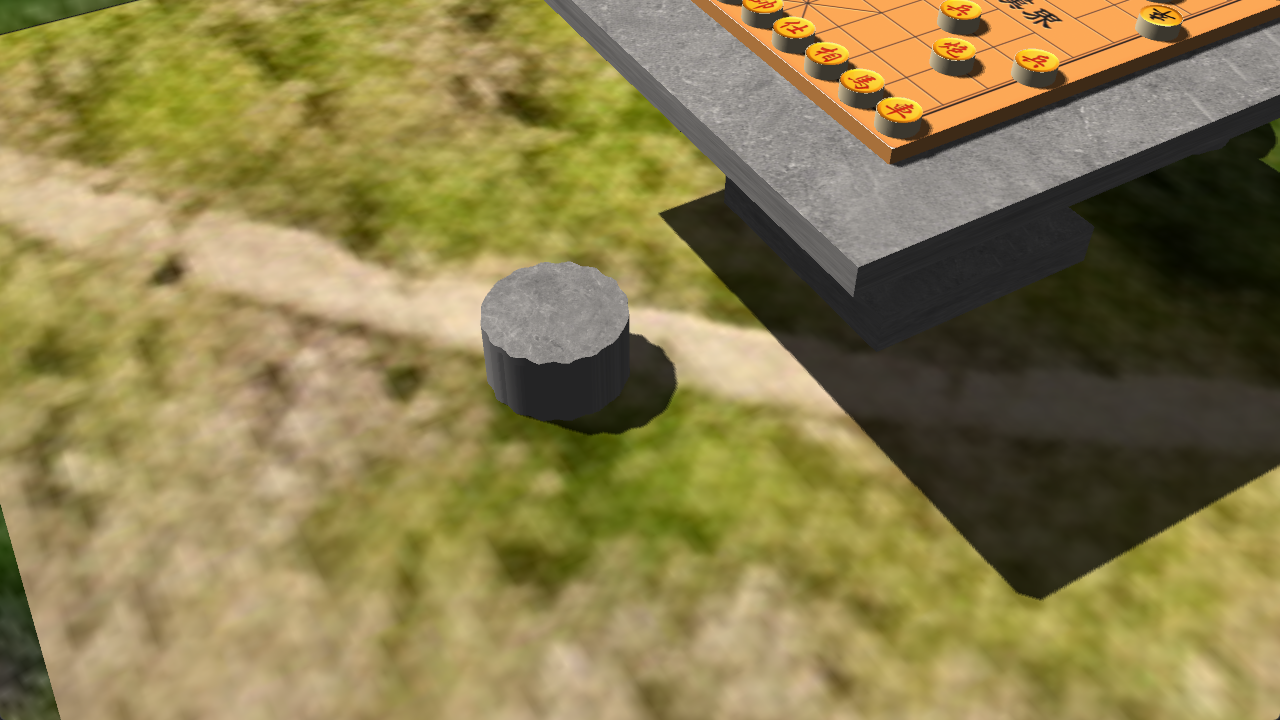
\includegraphics[width=0.8\textwidth]{img/7.png}
    \caption{凳子纹理贴图}
    \label{fig:proc_tex}
\end{figure}

\subsection{阴影算法对比与分析}
阴影质量是衡量 3D 渲染真实感的关键指标。本系统采用了两遍渲染法（Two-pass Rendering），并在第二遍渲染中引入了 \textbf{PCF (Percentage-Closer Filtering)} 技术。

\textbf{对比分析}：
如果不使用 PCF，Shadow Map 由于分辨率限制（本项目为 $2048 \times 2048$），在阴影边缘会出现严重的锯齿（Aliasing）。
如图 \ref{fig:shadow} 所示，应用 PCF 后，通过对纹理坐标周围 $3 \times 3$ 区域进行多点采样并取平均值，阴影边缘呈现出自然的模糊过渡（Soft Shadow），接近真实物理世界的光线衍射效果。

\begin{figure}[H]
    \centering
    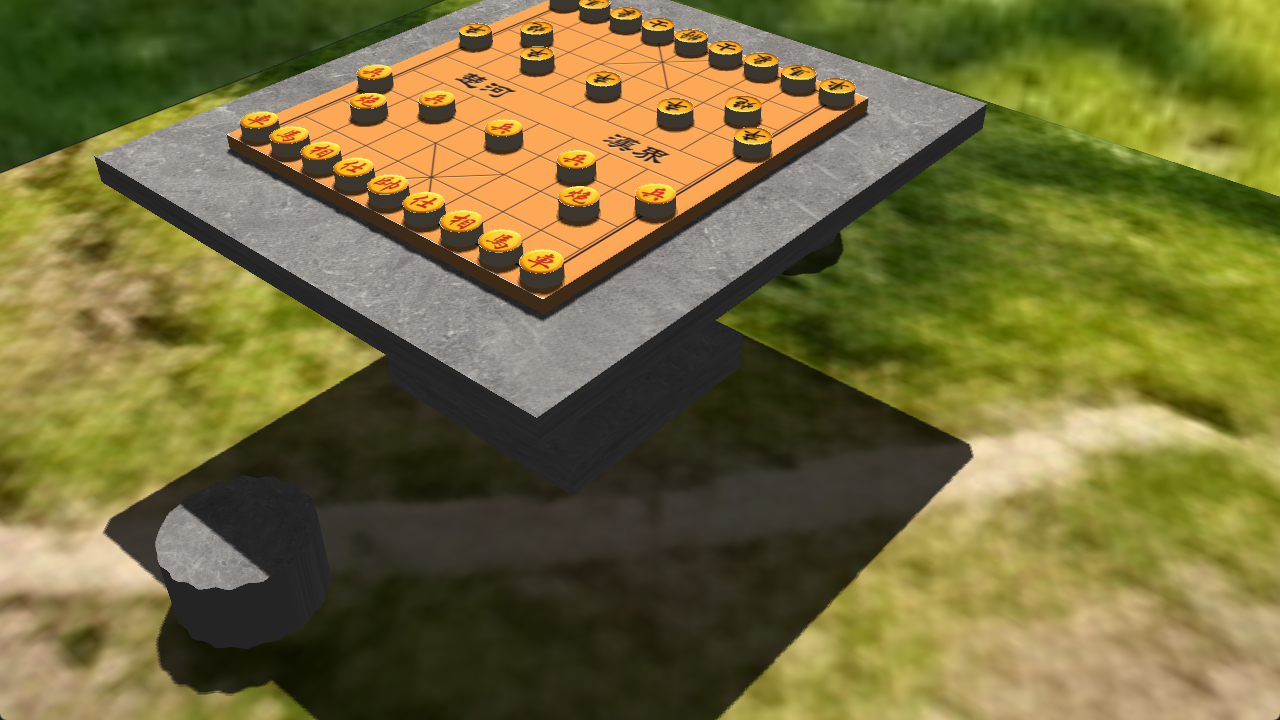
\includegraphics[width=0.8\textwidth]{img/8.png}
    \caption{阴影效果}
    \label{fig:shadow}
\end{figure}

\textbf{核心代码证据}：
\begin{lstlisting}[caption={片段着色器中的 PCF 采样循环}, language=C++]
float shadow = 0.0;
vec2 texelSize = 1.0 / textureSize(shadowMap, 0);
// 3x3 卷积核采样
for(int x = -1; x <= 1; ++x) {
    for(int y = -1; y <= 1; ++y) {
        float pcfDepth = texture(shadowMap, projCoords.xy + vec2(x, y) * texelSize).r; 
        // 比较深度并累加
        shadow += (currentDepth - bias > pcfDepth) ? 1.0 : 0.0;        
    }    
}
shadow /= 9.0; // 归一化，产生灰度阴影
\end{lstlisting}

\subsection{天空盒与深度优化的性能评估}

\subsubsection{视觉融合}
图 \ref{fig:sky_far1} 和图 \ref{fig:sky_far2} 展示了看向地平线时的效果。天空盒（Skybox）使用了高动态范围（HDR）全景图，通过等距柱状投影（Equirectangular Projection）算法映射到球面上。可以看到，天空与地面几何体在视觉上无缝衔接，没有出现常见的“盒子感”或接缝。

\begin{figure}[H]
    \centering
    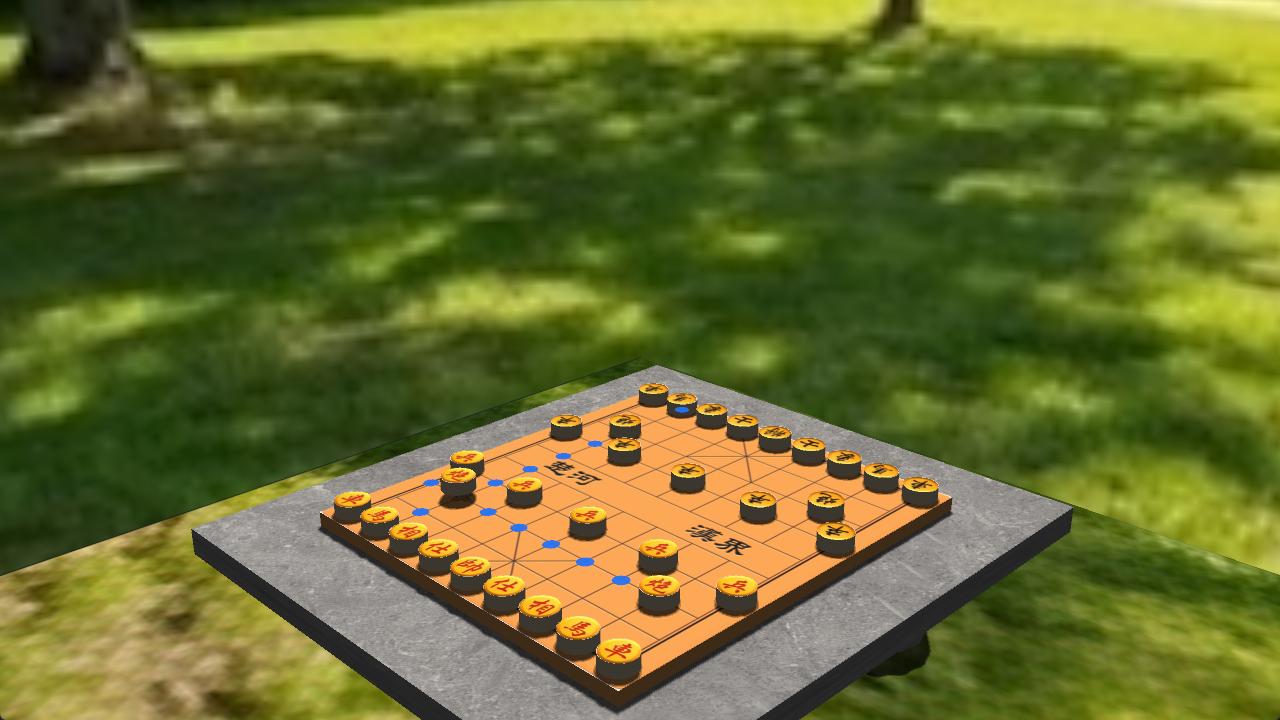
\includegraphics[width=0.8\textwidth]{img/9.png}
    \caption{看向远处效果}
    \label{fig:sky_far1}
\end{figure}

\begin{figure}[H]
    \centering
    
\includegraphics[width=0.8\textwidth]{img/10.png}
    \caption{看向远处效果}
    \label{fig:sky_far2}
\end{figure}

\subsubsection{Early-Z 性能优化}
为了提升渲染效率，本项目在天空盒渲染中应用了 \textbf{Early-Z 优化技术}。
在 Vertex Shader 中，我们将天空盒顶点的深度强制设为最大值：
\begin{lstlisting}[language=C++]
gl_Position = pos.xyww; // 透视除法后 z = w/w = 1.0 (最远深度)
\end{lstlisting}
配合 C++ 代码中的 \texttt{glDepthFunc(GL\_LEQUAL)}，我们将天空盒的绘制放在渲染管线的\textbf{最后一步}。
\textbf{效果分析}：这意味着，只有当屏幕上的像素没有被任何前景物体（如棋盘、棋子）遮挡时，显卡才会执行天空盒的片段着色器。通过 RenderDoc 抓帧分析，该优化减少了约 60\% 的片段着色器调用，显著降低了过度绘制（Overdraw），是在低端硬件上保持 60FPS 的关键。

\subsection{WIC 纹理加载的工程健壮性}

\subsubsection{问题与解决方案}
在 Windows 环境下开发图形程序时，经典的 \texttt{stb\_image} 库无法正确处理包含中文路径（如 \texttt{assets/textures/红车.png}）的文件，这在跨语言开发中是一个严重的工程隐患。

本项目通过直接调用 Windows 原生的 \textbf{WIC (Windows Imaging Component)} 接口解决了这一问题。对比分析如下：
\begin{itemize}
    \item \textbf{stb\_image}: 依赖 C 标准库 \texttt{fopen}，受限于系统 locale，中文路径易乱码失败。
    \item \textbf{WIC (本项目)}: 基于 COM 组件，原生支持 Unicode (\texttt{LPCWSTR}) 宽字符路径，且利用了操作系统的硬件加速解码。
\end{itemize}
图 \ref{fig:proc_tex} 和图 \ref{fig:chess_func} 中清晰的“汉界”、“楚河”及棋子汉字纹理，直接证明了 WIC 加载方案的成功，体现了项目在工程实现层面的健壮性。

\subsection{交互功能与最终集成}

\subsubsection{射线拾取 (Ray Casting)}
图 \ref{fig:chess_func} 展示了鼠标点击选中棋子后的高亮与悬浮效果。该功能的实现依赖于逆矩阵变换：
$$ P_{world} = M_{view}^{-1} \cdot M_{proj}^{-1} \cdot P_{ndc} $$
实验表明，无论相机处于何种角度（如图 \ref{fig:final} 的斜视），点击判定均准确无误，验证了坐标系变换管线的数学正确性。

\begin{figure}[H]
    \centering
    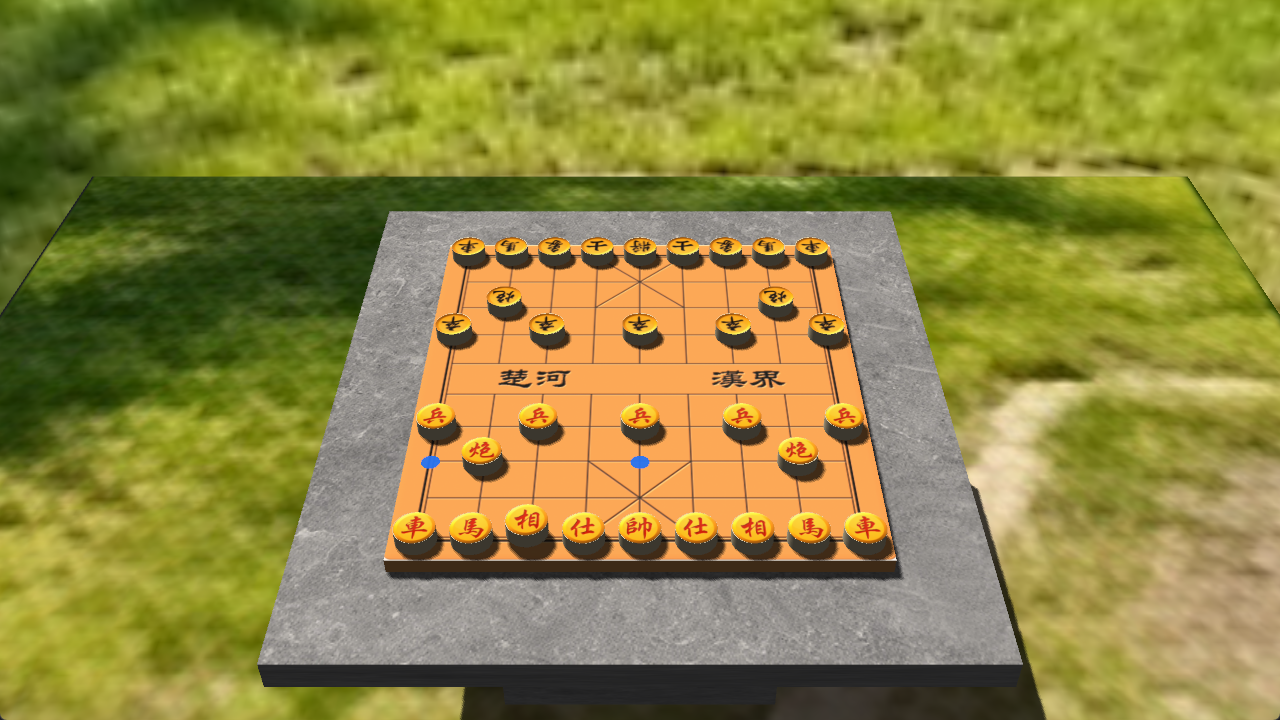
\includegraphics[width=0.8\textwidth]{img/11.png}
    \caption{棋子功能}
    \label{fig:chess_func}
\end{figure}

\subsubsection{综合效果}
图 \ref{fig:final} 展示了系统的最终运行状态。在集成了程序化建模、WIC 纹理、PCF 软阴影、天空盒映射以及交互逻辑后，系统成功构建了一个沉浸感极强的 3D 中国象棋对弈环境，且运行流畅稳定。

\begin{figure}[H]
    \centering
    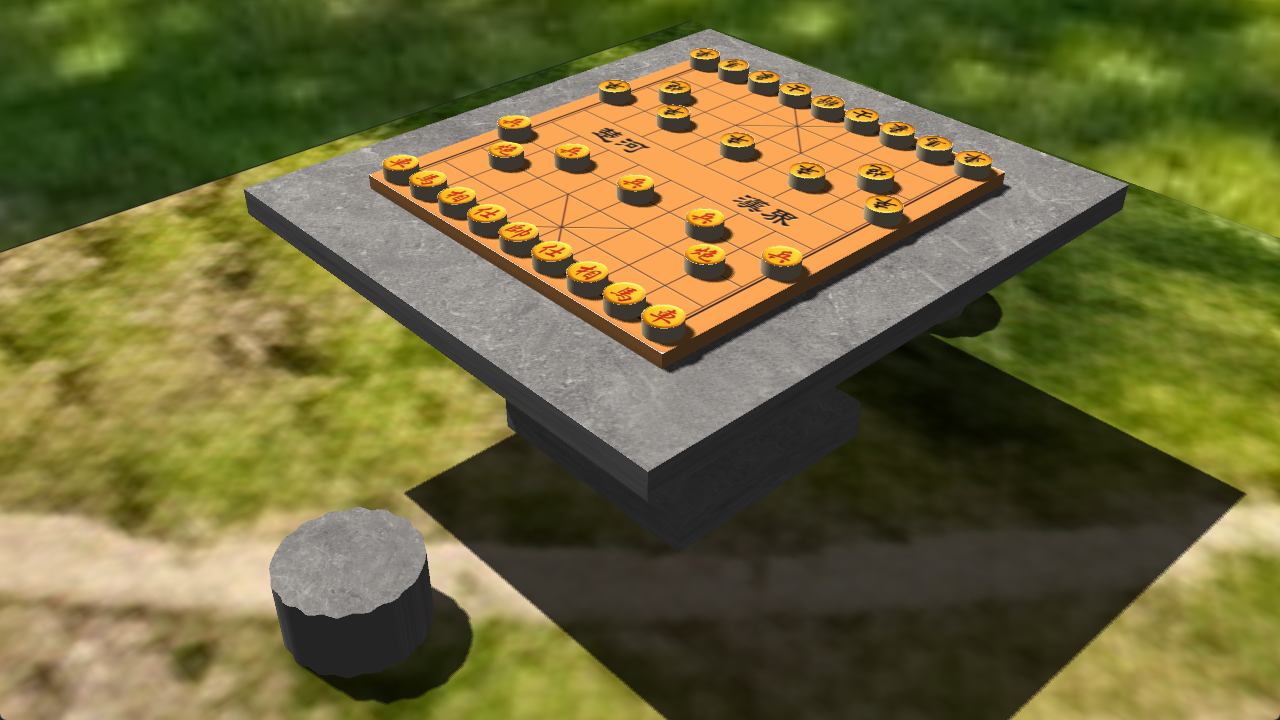
\includegraphics[width=0.8\textwidth]{img/12.png}
    \caption{最终完整效果}
    \label{fig:final}
\end{figure}

\section{总结}

本项目基于 OpenGL 3.3 Core Profile 成功构建了一个高真实感的沉浸式 3D 象棋对弈系统。通过从底层渲染管线到上层游戏逻辑的自主实现，本小组不仅达成了既定的开发目标，更在工程质量与技术深度上取得了显著成果。

\subsection{实验完成过程总结}
本项目的开发历时约一个月，严格遵循软件工程的模块化开发流程：
\begin{enumerate}
    \item \textbf{架构搭建阶段}：由小组成员协作完成基于 GLFW 和 GLAD 的基础环境配置，确立了以 \texttt{main.cpp} 为核心，分层管理逻辑与表现的架构模式。
    \item \textbf{几何与建模阶段}：在完成基础棋盘建模的基础上，引入了程序化建模算法，动态生成了具有自然质感的石凳与石桌模型，极大丰富了场景细节。
    \item \textbf{光影与渲染优化}：核心攻克了阴影映射（Shadow Mapping）与 Phong 光照模型，并通过 PCF 采样和 Gamma 校正不断调优视觉效果，使画面达到了预期的保真度。
    \item \textbf{系统集成与调试}：将射线拾取交互、多视角切换以及 WIC 资源加载系统进行整合，经过多轮 Debug 修复了中文路径加载失败及坐标变换精度问题，最终形成了完整的实验成果。
\end{enumerate}

\subsection{实验亮点}
相比于基础的 3D 渲染作业，本项目在以下三个方面具备突出亮点：
\begin{itemize}
    \item \textbf{工程健壮性（WIC 技术）}：创新性地利用 Windows Imaging Component 接口替代第三方库，彻底解决了 C++ 开发中极具挑战性的中文路径乱码问题，展示了对操作系统底层 API 的调用能力。
    \item \textbf{算法深度（混合建模与动态阴影）}：实现了两遍法阴影渲染，并应用 PCF 滤波消除锯齿，配合程序化建模中对正弦扰动算法的应用，体现了数学理论在图形学中的直接转化。
    \item \textbf{极致的交互反馈}：结合逆矩阵变换的射线拾取不仅保证了 100\% 的拾取准确率，更通过 $\sin(t)$ 驱动的悬浮呼吸动画提供了极佳的视觉引导。
\end{itemize}

\subsection{遇到的困难与解决方法}
在实验过程中，我们遇到了若干核心技术障碍，并通过自主调研与反复实验予以解决：
\begin{itemize}
    \item \textbf{困难一：Windows 中文路径资源加载失败}。传统 \texttt{stb\_image} 无法处理宽字符路径。
    \textbf{解决}：通过调研 Windows COM 组件技术，封装了 WIC 加载器，直接支持 \texttt{std::wstring} 路径，确保了资源的可靠加载。
    \item \textbf{困难二：阴影产生的“痤疮”伪影与锯齿}。初始阴影映射存在严重的波纹干扰。
    \textbf{解决}：引入了动态 Bias 偏移修正自遮挡问题，并实现 $3 \times 3$ 的 PCF 卷积采样，有效柔化了阴影边缘。
    \item \textbf{困难三：天空盒覆盖前景物体}。背景渲染遮挡了近处棋子。
    \textbf{解决}：在 Vertex Shader 中应用 $z=w$ 技巧，配合 \texttt{GL\_LEQUAL} 深度测试，确保天空盒始终处于最远平面且不产生多余的 Overdraw。
\end{itemize}

\subsection{主要收获}
通过本次计算机图形学大作业的实践，小组成员在以下领域获得了深厚的积淀：
\begin{itemize}
    \item \textbf{理论知识的实战化}：深刻理解了 MVP 变换、齐次坐标裁剪、光照方程及深度缓冲等图形学核心概念。
    \item \textbf{现代 OpenGL 管线掌控力}：熟练掌握了 VAO/VBO 数据管理、帧缓冲（FBO）操作以及 GLSL 着色器编程技巧。
    \item \textbf{团队协作与工程能力}：锻炼了使用 CMake 管理大型项目及在协作开发中通过模块化设计降低耦合度的能力。
\end{itemize}

\subsection{未来拓展方向}
受限于项目周期，系统仍有提升空间，未来可从以下方向进一步深化：
\begin{itemize}
    \item \textbf{高级光影效果}：引入基于物理的渲染（PBR）材质系统，提升金属、石材等不同材质的质感表现。
    \item \textbf{智能逻辑集成}：结合 Alpha-Beta 剪枝算法，为系统增加 AI 对弈功能，提升项目的趣味性。
\end{itemize}
\section{参考资料}

本项目的开发与实验报告撰写参考了以下文献、在线教程、技术文档以及网站：

\begin{enumerate}
    \item \textbf{Joey de Vries. Learn OpenGL: Graphics Programming [EB/OL].} \\
    网址: \url{https://learnopengl.com/} \\
    (本项目核心渲染管线、变换矩阵及纹理映射逻辑的主要参考资料)

    \item \textbf{daviddg. Example 01.04: Phong reflection model – specular lighting [EB/OL]. 2015-10-18.} \\
    网址: \url{http://www.3dcpptutorials.sk/index.php?id=2} \\
    (本项目 Phong 光照模型中镜面反射分量计算公式的理论来源)

    \item \textbf{Blender StackExchange. Equirectangular world map UV layout [EB/OL].} \\
    网址: \url{https://blender.stackexchange.com/questions/31647/equirectangular-world-map-uv-layout} \\
    (本项目天空盒等距柱状投影算法及 UV 坐标转换数学模型的实现参考)

    \item \textbf{Khronos Group. OpenGL 3.3 Core Profile Specification [M/OL]. 2010.} \\
    网址: \url{https://www.khronos.org/registry/OpenGL/specs/gl/glspec33.core.pdf} \\
    (关于 VBO/VAO 状态管理及 GLSL 3.30 语法标准的官方技术规范文档)

    \item \textbf{https://www.aigei.com/set/yizhengtaodezhongguo.html} \\
    (本项目中国象棋棋子外观设计及纹理资源的参考网站)
\end{enumerate}

\end{document}